\section{Experiments}
\label{sec:exp}

\noindent\textbf{Datasets and protocol.} Mip-NeRF~360~\cite{barron2022mipnerf360} (9 scenes), Tanks and Temples~\cite{knapitsch2017tanks} (truck, train), NeRF-Synthetic~\cite{mildenhall2020nerf} (8 objects) and Deep Blending~\cite{hedman2018deep} (drjohnson, playroom). Deep Blending was not used while developing the method; every number on it comes from one run with the settings fixed on the other datasets. \MS training is unchanged (30k iterations, images downsampled by 2 indoors and by 4 outdoors, the standard test split, black background for NeRF-Synthetic). Quality is PSNR, SSIM and LPIPS of the \emph{decoded file} rendered at the renderer's supersampling; all sizes are bytes of the single delivered file. The \emph{FP32 model} is the trained \MS mesh in 32-bit floats, our reproduction; it is the reference for compression ratios and quality loss. One configuration for all scenes: appearance dictionary $4096+256$, position grid of 14--18 bits by scene extent, 7-bit DC color, growth aim $\alpha=1.25$ for captured scenes and $1.1$ for synthetic objects, collapse rounds every 500 iterations from 12.5k to 19.5k. ``At the same vertex count'' means after \MS's final cleaning.

\subsection{Size must be decided during training}
\label{sec:e1}
Table~\ref{tab:cap} answers the two questions a reader will ask first. \emph{Why not decimate a trained mesh?} For each scene and three vertex counts (those of \BM's own 20 / 10 / 5~MB files; 4 / 2.5 / 1.5~MB on NeRF-Synthetic) we compare \MS trained with that count as a vertex cap against the FP32 model simplified to the same count by edge collapse (quadric error with an appearance term) followed by the same 3000-step fine-tuning, both through our codec. Training to the count wins on 62 of 63 pairs, by 1.85\dB on average and by up to 5.5\dB; the gap grows as the budget shrinks (0.5\dB at the largest, 3.8\dB at the smallest count on real scenes). The simplified meshes keep fewer faces per vertex and show holes and speckle (Fig.~\ref{fig:qual}, right). \emph{Is the growth rule itself better than a vertex cap?} Against \MS trained with the cap set from \BM's own vertex count (pairs within $\pm15\%$), rate-aware growth is better on 44 of 45 pairs, by 0.27\dB on real scenes and 0.24\dB on objects, measured on the FP32 meshes \emph{before any entropy coding}; the margin is unchanged after the codec, so it belongs to the growth rule, not to the encoder. At the same file size after the codec the margin is 0.21\dB on real scenes (30/33); on NeRF-Synthetic it is 0.12\dB (16/24) because the 4~MB group contains three objects at their capacity limit (Sec.~\ref{sec:e3}); at 1.5~MB it is 0.24\dB on 8 of 8.

\begin{table}[t]\centering\small
\caption{\textbf{Deciding the size during training.} Top: \MS trained with a vertex cap vs.\ the FP32 model simplified after training to the same vertex count, both through our codec (PSNR gain of training, dB; count of pairs where training is better). Bottom: \BM vs.\ \MS trained with a vertex cap, at the same vertex count without any entropy coding (FP32 meshes), the same after our codec, and at the same file size after our codec. Three vertex counts / sizes per scene. Deep Blending rows use the controller-free growth runs of our development set (stated).}
\label{tab:cap}
\setlength{\tabcolsep}{4pt}
\begin{tabular}{lrrr}
\toprule
\multicolumn{4}{l}{\emph{Training with a vertex cap vs.\ simplification after training}} \\
Dataset & pairs & mean gain & range \\
\midrule
Mip-NeRF 360 + T\&T & 33 & $+2.07$ (33/33) & $+0.10$ to $+5.48$ \\
NeRF-Synthetic & 24 & $+1.33$ (23/24) & $-0.03$ to $+4.35$ \\
Deep Blending & 6 & $+2.71$ (6/6) & $+1.39$ to $+4.72$ \\
\midrule
\multicolumn{4}{l}{\emph{\BM vs.\ \MS with a vertex cap}} \\
Dataset & same $V$, no codec & same $V$, codec & same file size \\
\midrule
Mip-NeRF 360 + T\&T & $+0.27$ (29/30) & $+0.26$ (29/30) & $+0.21$ (30/33) \\
NeRF-Synthetic & $+0.24$ (15/15) & $+0.22$ (15/15) & $+0.12$ (16/24) \\
Deep Blending & $+0.15$ (5/6) & -- & $+0.19$ (5/6) \\
\bottomrule
\end{tabular}
\end{table}

\subsection{Size as an input}
\label{sec:e3}
Table~\ref{tab:size} reports, per dataset and target, the mean file size, the size error $(\text{file size}-\text{target})/\text{target}$ and the count of scenes within $\pm10\%$; Fig.~\ref{fig:rd} draws the same runs as rate--distortion curves, with the per-scene spread of the landing as whiskers at each target. Across the four datasets 83 of 89 runs land within $\pm10\%$ with one setting per capture class. The misses are systematic and we report them: indoor scenes land 5--14\% above the target (kitchen at 10~MB is the worst, $+13.5\%$), because the visible-face set keeps growing after the growth phase and the collapse rounds can remove only so much per round; outdoor scenes at 20~MB land up to 7\% below, because the last growth step admits fewer splits than planned and nothing can add vertices afterwards. On NeRF-Synthetic several objects cannot fill 3--6~MB at all: the price falls to its floor from the first steps and the file stays small (ficus, mic; six of eight objects at 6~MB). These \emph{capacity-limited} runs are counted separately and never hidden. Deep Blending, untouched during development, lands at $+7$ to $+10\%$ on average: the same indoor behaviour as Mip-NeRF~360, no retuning.

\noindent\textbf{Cost of control.} The best a growth rule can do at a given file size is what it reaches when the size is \emph{not} prescribed: the same rule run at a fixed price, several trainings per scene, the size read off afterwards. Against that reference curve (three fixed prices per scene, landing at about 5, 12 and 25~MB on real scenes and 1.5, 2.5 and 4~MB on objects), \BM is $0.04$\dB lower at 20~MB, $0.06$\dB at 2.5~MB and $0.02$\dB at 1.5~MB, where a fixed-price run lands at about the same size as the target, and $0.13$\dB lower at 10~MB, where the curve is read between two prices (the curve is concave, so this chord reading under-estimates the cost; the three points bound the error at $0.19$\dB on average over a span twice as wide). The cost of getting the size in one training is therefore below $0.1$\dB where it can be measured directly and below about $0.3$\dB everywhere. Run-to-run variance of the full method, three seeds on four scenes: the file size moves by 0.5--5\% of the target and the PSNR by 0.01--0.14\dB. The reference also shows why a price is not a size: at one fixed price the file size varies by $2.2$--$2.5\times$ across the 11 real scenes (4.7--11.7~MB at one price, 10.8--24.0~MB at another).

\begin{table}[t]\centering\small
\setlength{\tabcolsep}{2.6pt}
\caption{\textbf{Size error and quality per dataset and target.} Mean file size, size error (mean; range), scenes within $\pm10\%$, PSNR of the decoded files with its change against the FP32 model, SSIM and LPIPS; means over the scenes below the capacity limit (capacity-limited objects in parentheses). The 15, 7.5 and 3~MB targets are in the supplement.}
\label{tab:size}
\begin{tabular}{@{}llrrrrr@{}}
\toprule
dataset & target & MB & size error & $\pm10\%$ & PSNR ($\Delta$) & SSIM / LPIPS \\
\midrule
\multirow{3}{*}{\shortstack[l]{Mip-NeRF 360\\+ T\&T (11)}} & 20 MB & 19.9 & $-0.5\%$ ($-6.6$..$+10.0$) & 10 & 23.75 ($-0.30$) & 0.712 / 0.397 \\
 & 10 MB & 10.2 & $+2.0\%$ ($-4.7$..$+13.5$) & 10 & 23.39 ($-0.66$) & 0.684 / 0.442 \\
 & 5 MB & 5.0 & $+0.6\%$ ($-4.8$..$+9.2$) & 11 & 22.72 ($-1.32$) & 0.644 / 0.491 \\
\midrule
\multirow{3}{*}{\shortstack[l]{Deep\\Blending (2)}} & 20 MB & 21.3 & $+6.7\%$ ($+3.6$..$+9.7$) & 2 & 26.94 ($-0.28$) & 0.838 / 0.452 \\
 & 10 MB & 11.0 & $+10.2\%$ ($+8.3$..$+12.0$) & 1 & 26.54 ($-0.69$) & 0.830 / 0.478 \\
 & 5 MB & 5.4 & $+7.9\%$ ($+4.7$..$+11.1$) & 1 & 25.89 ($-1.34$) & 0.817 / 0.502 \\
\midrule
\multirow{3}{*}{\shortstack[l]{NeRF-\\Synthetic (8)}} & 4 MB & 3.9 & $-2.9\%$ ($-10.3$..$+3.4$) & 5 (+2) & 30.60 ($-0.13$) & 0.942 / 0.082 \\
 & 2.5 MB & 2.6 & $+2.6\%$ ($-6.6$..$+9.2$) & 7 (+1) & 30.81 ($-0.30$) & 0.947 / 0.076 \\
 & 1.5 MB & 1.6 & $+4.0\%$ ($+1.0$..$+9.0$) & 8 & 30.36 ($-0.88$) & 0.944 / 0.080 \\
\bottomrule
\end{tabular}
\end{table}

\begin{figure*}[t]\centering
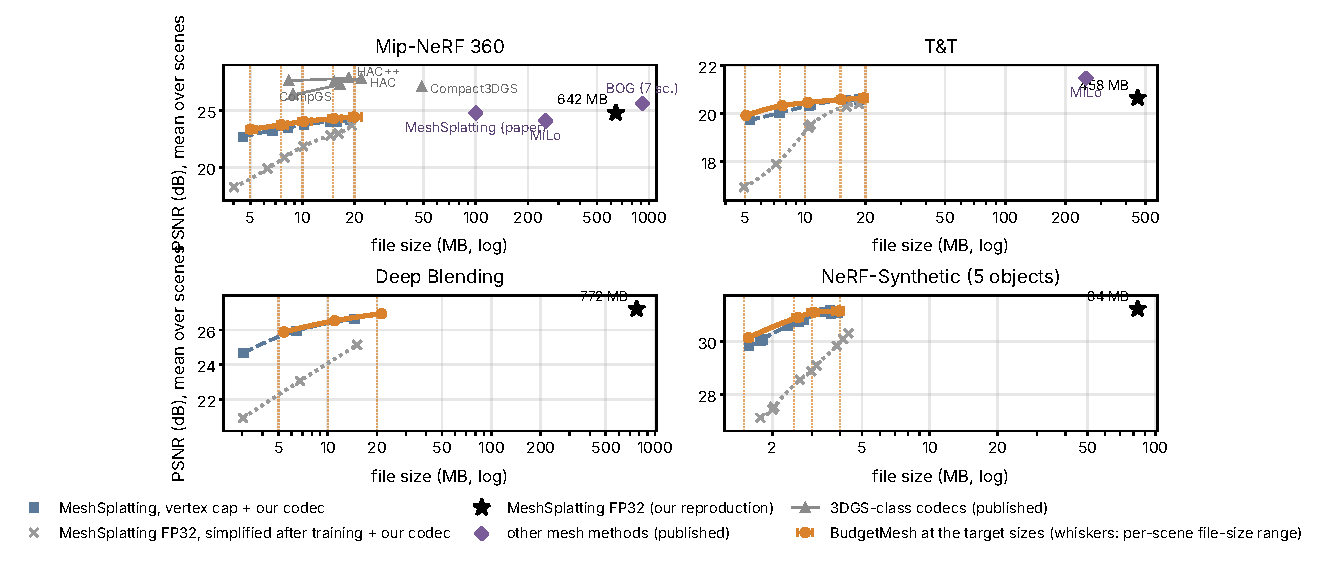
\includegraphics[width=\textwidth]{figures/fig_rd_per_dataset.pdf}
\caption{\textbf{Rate--distortion per dataset.} Mean PSNR vs.\ mean file size over the dataset's scenes. Orange: \BM at each target size, the dotted vertical lines are the targets and the whiskers the per-scene range of the delivered file size (the landing is tight enough that most whiskers are shorter than the marker). Blue: \MS trained with a vertex cap and encoded with the same codec. Star: the FP32 model. Diamonds: published mesh-output methods at their own asset sizes. Grey triangles (Mip-NeRF~360): published 3DGS-class codecs, 3--4\dB above us at the same size (Sec.~\ref{sec:e4}). NeRF-Synthetic shows the five objects below their capacity limit at every target. Curves are monotone interpolations of the measured points.}
\label{fig:rd}
\end{figure*}

\subsection{Compression results and other representations}
\label{sec:e4}
Table~\ref{tab:cross} puts \BM next to published mesh-output methods and 3DGS-class codecs on the three captured datasets. Against the FP32 model the 20, 10 and 5~MB files are 31$\times$, 60$\times$ and 122$\times$ smaller at $-0.30$, $-0.66$ and $-1.32$\dB on real scenes (Table~\ref{tab:size}); against the same meshes written as a quantised PLY and compressed with zstd, the honest ``trivial'' baseline, they are 7$\times$, 14$\times$ and 27$\times$ smaller. The ratio splits into two factors: the file holds fewer vertices than the FP32 model (1.4$\times$, 3.0$\times$ and 6.7$\times$ fewer at 20, 10 and 5~MB; the FP32 meshes have 1.9--3.2M vertices) and each vertex costs fewer bytes (231 bytes in FP32 against 11--13 in our file, 18--21$\times$); the first factor is the growth rule's, the second the codec's. Within the mesh class ours is the only entry below 100~MB: 5--45$\times$ smaller than the published assets, 0.3\dB below \MS's own file and 1.2\dB below Binary Opacity Grids at 20~MB, above MiLo, RaDe-GS and GOF. Against 3DGS-class codecs the table says what the figure shows: at 5--20~MB HAC++ and HAC are 3.3--4\dB above us on all three datasets, with a smaller SSIM gap (0.10--0.11) and a larger LPIPS gap (0.16--0.21). That gap is the representation's, opaque triangles against anisotropic Gaussians, and this paper is about what the mesh class can do per byte; it buys a standard mesh that renders in any engine (145--350~fps on an iPhone~17~Pro at capture resolution with a vertex shader) and decodes in 2.3--6.4~s on one CPU core. SSIM and LPIPS degrade faster than PSNR as the budget shrinks (LPIPS 0.31 for FP32, 0.40 at 20~MB, 0.49 at 5~MB on Mip-NeRF~360); Sec.~\ref{sec:e6} traces this to the shared appearance dictionary.

\begin{table*}[t]\centering\small
\setlength{\tabcolsep}{3.2pt}
\caption{\textbf{Against other representations}, published numbers at each method's own reported asset size (3DGS-class rows from the HAC++ paper's table; mesh-class rows from the respective papers; MiLo, RaDe-GS and GOF are Gaussian methods with a mesh output; Binary Opacity Grids reports the 7-scene Mip-NeRF~360 subset). \BM rows are means over the decoded files at each target. $^{a}$\MS's RGB-only PLY (the 100~MB figure); its full model is our FP32 reproduction row. Sizes in MB.}
\label{tab:cross}
\begin{tabular}{llrrrrrrrrrrrr}
\toprule
 & & \multicolumn{4}{c}{Mip-NeRF 360} & \multicolumn{4}{c}{Tanks and Temples} & \multicolumn{4}{c}{Deep Blending} \\
\cmidrule(lr){3-6}\cmidrule(lr){7-10}\cmidrule(lr){11-14}
 & method & PSNR & SSIM & LPIPS & size & PSNR & SSIM & LPIPS & size & PSNR & SSIM & LPIPS & size \\
\midrule
\multirow{9}{*}{\rotatebox{90}{Gaussian splats}}
 & 3DGS~\cite{kerbl2023gaussians} & 27.46 & 0.812 & 0.222 & 750.9 & 23.69 & 0.844 & 0.178 & 431.0 & 29.42 & 0.899 & 0.247 & 663.9 \\
 & Scaffold-GS~\cite{scaffold2024} & 27.50 & 0.806 & 0.252 & 253.9 & 23.96 & 0.853 & 0.177 & 86.5 & 30.21 & 0.906 & 0.254 & 66.0 \\
 & Compact3DGS~\cite{compact3dgs2024} & 27.08 & 0.798 & 0.247 & 48.8 & 23.32 & 0.831 & 0.201 & 39.4 & 29.79 & 0.901 & 0.258 & 43.2 \\
 & LightGaussian~\cite{lightgaussian2024} & 27.00 & 0.799 & 0.249 & 44.5 & 22.83 & 0.822 & 0.242 & 22.4 & 27.01 & 0.872 & 0.308 & 33.9 \\
 & HAC~\cite{hac2024} (low / high rate) & 27.53 / 27.77 & 0.807 / 0.811 & 0.238 / 0.230 & 15.3 / 21.9 & 24.04 / 24.40 & 0.846 / 0.853 & 0.187 / 0.177 & 8.1 / 11.2 & 29.98 / 30.34 & 0.902 / 0.906 & 0.269 / 0.258 & 4.4 / 6.4 \\
 & CompGS~\cite{compgs2024} (low / high) & 26.37 / 27.26 & 0.778 / 0.803 & 0.276 / 0.239 & 8.8 / 16.5 & 23.11 / 23.70 & 0.815 / 0.837 & 0.236 / 0.208 & 5.9 / 9.6 & 29.30 / 29.69 & 0.895 / 0.901 & 0.293 / 0.279 & 6.0 / 8.8 \\
 & HAC++~\cite{hacpp2025} (low / high) & 27.60 / 27.82 & 0.803 / 0.811 & 0.253 / 0.231 & 8.3 / 18.5 & 24.22 / 24.32 & 0.849 / 0.854 & 0.190 / 0.178 & 5.2 / 8.6 & 30.16 / 30.34 & 0.907 / 0.911 & 0.266 / 0.254 & 2.9 / 5.3 \\
\midrule
\multirow{6}{*}{\rotatebox{90}{opaque meshes}}
 & \MS~\cite{meshsplatting2025} (paper) & 24.78 & 0.728 & 0.310 & 100$^a$ & 20.52 & 0.745 & 0.287 & -- & -- & -- & -- & -- \\
 & \MS FP32 (our reproduction) & 24.81 & 0.731 & 0.309 & 642 & 20.64 & 0.760 & 0.272 & 459 & 27.23 & 0.842 & 0.337 & 772 \\
 & MiLo~\cite{milo2025} & 24.09 & 0.688 & 0.323 & 253 & 21.46 & 0.706 & 0.348 & -- & -- & -- & -- & -- \\
 & Binary Opacity Grids~\cite{bog2024} (7 sc.) & 25.62 & -- & -- & 913 & -- & -- & -- & -- & -- & -- & -- & -- \\
 & RaDe-GS mesh~\cite{rade2024} & 23.56 & 0.668 & 0.361 & 1100 & 20.51 & 0.659 & 0.344 & -- & -- & -- & -- & -- \\
 & GOF mesh~\cite{gof2024} & 20.78 & 0.573 & 0.465 & 1500 & 21.69 & 0.690 & 0.326 & -- & -- & -- & -- & -- \\
\midrule
\multirow{3}{*}{\rotatebox{90}{ours}}
 & \BM, 20 MB target & 24.44 & 0.704 & 0.411 & 20.0 & 20.64 & 0.748 & 0.337 & 19.6 & 26.94 & 0.838 & 0.452 & 21.3 \\
 & \BM, 10 MB target & 24.04 & 0.673 & 0.458 & 10.2 & 20.45 & 0.731 & 0.368 & 10.3 & 26.54 & 0.830 & 0.478 & 11.0 \\
 & \BM, 5 MB target & 23.35 & 0.632 & 0.508 & 5.0 & 19.91 & 0.696 & 0.416 & 5.1 & 25.89 & 0.817 & 0.502 & 5.4 \\
\bottomrule
\end{tabular}
\end{table*}

\subsection{Against generic mesh codecs}
\label{sec:e5}
Could an off-the-shelf mesh codec replace ours? Table~\ref{tab:generic} runs the same FP32 meshes through Draco~\cite{draco}, the MPEG SC3DMC/TFAN coder~\cite{mamou2009tfan} and zstd, and compares bytes with our file for the same mesh (our encoder at its top operating point, $-0.1$ to $-0.8$\dB). Keeping view dependence as 8-bit SH attributes, Draco needs 12--18$\times$ and MPEG 3--4$\times$ our bytes; the only generic routes near our size drop the SH altogether (RGB-only vertex colors, or a baked texture) and lose 0.7--4.4\dB. The generic rows are near-lossless and ours is not, so the table measures the bytes each coder needs for essentially the same mesh rather than a rate--distortion curve; The fair generic point is Draco carrying exactly our appearance payload, the two dictionary indices and the 7-bit DC color as one generic attribute on the same positions and faces: its file is $2.7$--$3.5\times$ ours on every real-scene asset ($2.1$--$3.5\times$ on objects), and Draco's geometry alone, positions and connectivity with no appearance at all, already weighs $0.85$--$1.24\times$ our whole file. Our appearance streams cost 18--42\% of our file; coded by Draco's attribute predictor they cost two to three files. Our meshes are triangle soups stitched late in training and are not manifold, which is what the Edgebreaker-style coders pay for; the mesh statistics are in the supplement.

\begin{table}[t]\centering\small
\setlength{\tabcolsep}{3pt}
\caption{\textbf{Generic codecs on the same mesh.} File size of each route divided by ours, range over the 11 Mip-NeRF~360 / T\&T scenes (mean); quality loss against FP32. ``Ours'' is the top operating point of our encoder on the same mesh.}
\label{tab:generic}
\begin{tabular}{@{}lrrc@{}}
\toprule
route & size $\div$ ours & $\Delta$PSNR & view dep. \\
\midrule
Draco + 8-bit SH & 12.3--17.7$\times$ (15.0) & $-0.02$..$-0.21$ & yes \\
MPEG TFAN + 8-bit SH (10 sc.) & 3.0--4.2$\times$ (3.7) & $-0.02$..$-0.21$ & yes \\
quantised PLY + zstd & 4.4--6.2$\times$ (5.2) & $-0.02$..$-0.21$ & yes \\
Draco + our indices (generic attr.) & 2.7--3.5$\times$ (3.0) & $=$ ours & yes \\
Draco geometry + our indices via zstd & 1.3--1.6$\times$ (1.4) & $=$ ours & yes \\
Draco geometry only (no appearance) & 0.85--1.24$\times$ (1.05) & -- & no \\
Draco + 8-bit RGB & 1.8--2.4$\times$ (2.1) & $-0.7$..$-4.4$ & no \\
baked $4096^2$ texture + Draco geometry & 2.4--3.2$\times$ (2.7) & $-0.7$..$-4.4$ & no \\
ours & 1$\times$ & $-0.1$..$-0.8$ & yes \\
\bottomrule
\end{tabular}
\end{table}

\subsection{Where the bytes go}
\label{sec:e6}
Splitting a file into its streams (figure in the supplement): connectivity is 39--43\% and lossless, positions 20\%, appearance indices 17--20\%, DC color 11--13\%, and the dictionaries a fixed 0.65~MB (3\% of a 20~MB file, 12\% of a 5~MB one). Two findings follow. \emph{Appearance sharing carries the loss:} 45 of the 52 floats per vertex are SH, replaced by two indices; at the top operating point an 8-bit instead of 7-bit DC color recovers only 0.04--0.08\dB of the 0.4--0.6\dB loss on indoor scenes, so the remainder is the dictionary, and so is the LPIPS increase of Table~\ref{tab:cross}. \emph{Dictionary size should follow vertex count:} over a sweep of dictionary sizes and prices on all 21 scenes, the fixed $4096+256$ is within 0.16\dB of the best choice at every point on captured scenes, but on the two smallest objects (mic, ficus) a 1024-entry dictionary at a lower price is $+0.5$--$0.6$\dB at the same file size. The sweep is in the supplement; the paper uses the fixed setting.



\subsection{Ablation}
\label{sec:e7}
Table~\ref{tab:abl} switches off one part of the training rule at a time on all 11 real scenes at 10~MB and all NeRF-Synthetic objects at 2.5~MB, same code, codec and evaluation (ficus is capacity-limited at 2.5~MB and excluded). At 10--20~MB on real scenes the growth plan alone lands within 10\% on 9--10 of 11 scenes and none of the parts changes the quality at the same file size by more than 0.03\dB; the collapse rounds and the byte probe each remove one failure mode. The collapse trims the indoor overshoot (kitchen $+20\%\rightarrow+13\%$; on objects it takes the hit rate from 2/7 to 7/7). The probe is what makes small files land: with the fixed constants the 1.5~MB objects land $+18\%$ on average, 1 of 8 within 10\%, against $+4\%$ and 8 of 8 with the probe, while at 20~MB the constants are within 10\% on 10 of 11. The last row is the one that supports Sec.~\ref{sec:e1}: with the number of splits per step copied from the full run, choosing the triangles by \MS's importance score instead of error per byte gives meshes that \MS's own pruning then cuts further, and at the same file size they are 0.42\dB worse on every real scene and 0.24\dB worse on objects.

\begin{table}[t]\centering\small
\caption{\textbf{Ablation.} Size error (mean; scenes within $\pm10\%$) and quality at the same file size relative to the full method, read on each scene's reference curve of three fixed prices ($\Delta$PSNR; scenes where the variant is better). Mip-NeRF~360 / T\&T at 10~MB (11 scenes), NeRF-Synthetic at 2.5~MB (7 objects; ficus is capacity-limited). The fixed-constants variant was also run at 20~MB ($+3.4\%$, 10/11, $+0.03$\dB) and 1.5~MB ($+17.9\%$, 1/8, $+0.05$\dB).}
\label{tab:abl}
\setlength{\tabcolsep}{2.5pt}
\begin{tabular}{@{}lrrrr@{}}
\toprule
 & \multicolumn{2}{c}{real scenes, 10 MB} & \multicolumn{2}{c}{objects, 2.5 MB} \\
\cmidrule(lr){2-3}\cmidrule(lr){4-5}
variant & size err. & $\Delta$PSNR & size err. & $\Delta$PSNR \\
\midrule
full \BM & $+2.0\%$ (10/11) & 0 & $+2.6\%$ (7/7) & 0 \\
no in-training collapse & $+4.5\%$ (9/11) & $-0.03$ (4/11) & $+9.0\%$ (2/7) & $-0.05$ (3/7) \\
no byte probe (constants) & $+5.0\%$ (10/11) & $+0.03$ (9/11) & $+12.8\%$ (1/7) & $+0.07$ (6/7) \\
\MS's selection, same counts & $-27\%$ (0/11) & $-0.42$ (0/11) & $-11\%$ (4/7) & $-0.24$ (1/7) \\
\bottomrule
\end{tabular}
\end{table}

\subsection{Qualitative results}
\label{sec:e8}
Fig.~\ref{fig:qual} shows decoded files at the three main targets next to the ground truth and the FP32 model, with an enlarged crop and the error map per column, and the same vertex count reached three ways on one view.

\begin{figure*}[t]\centering
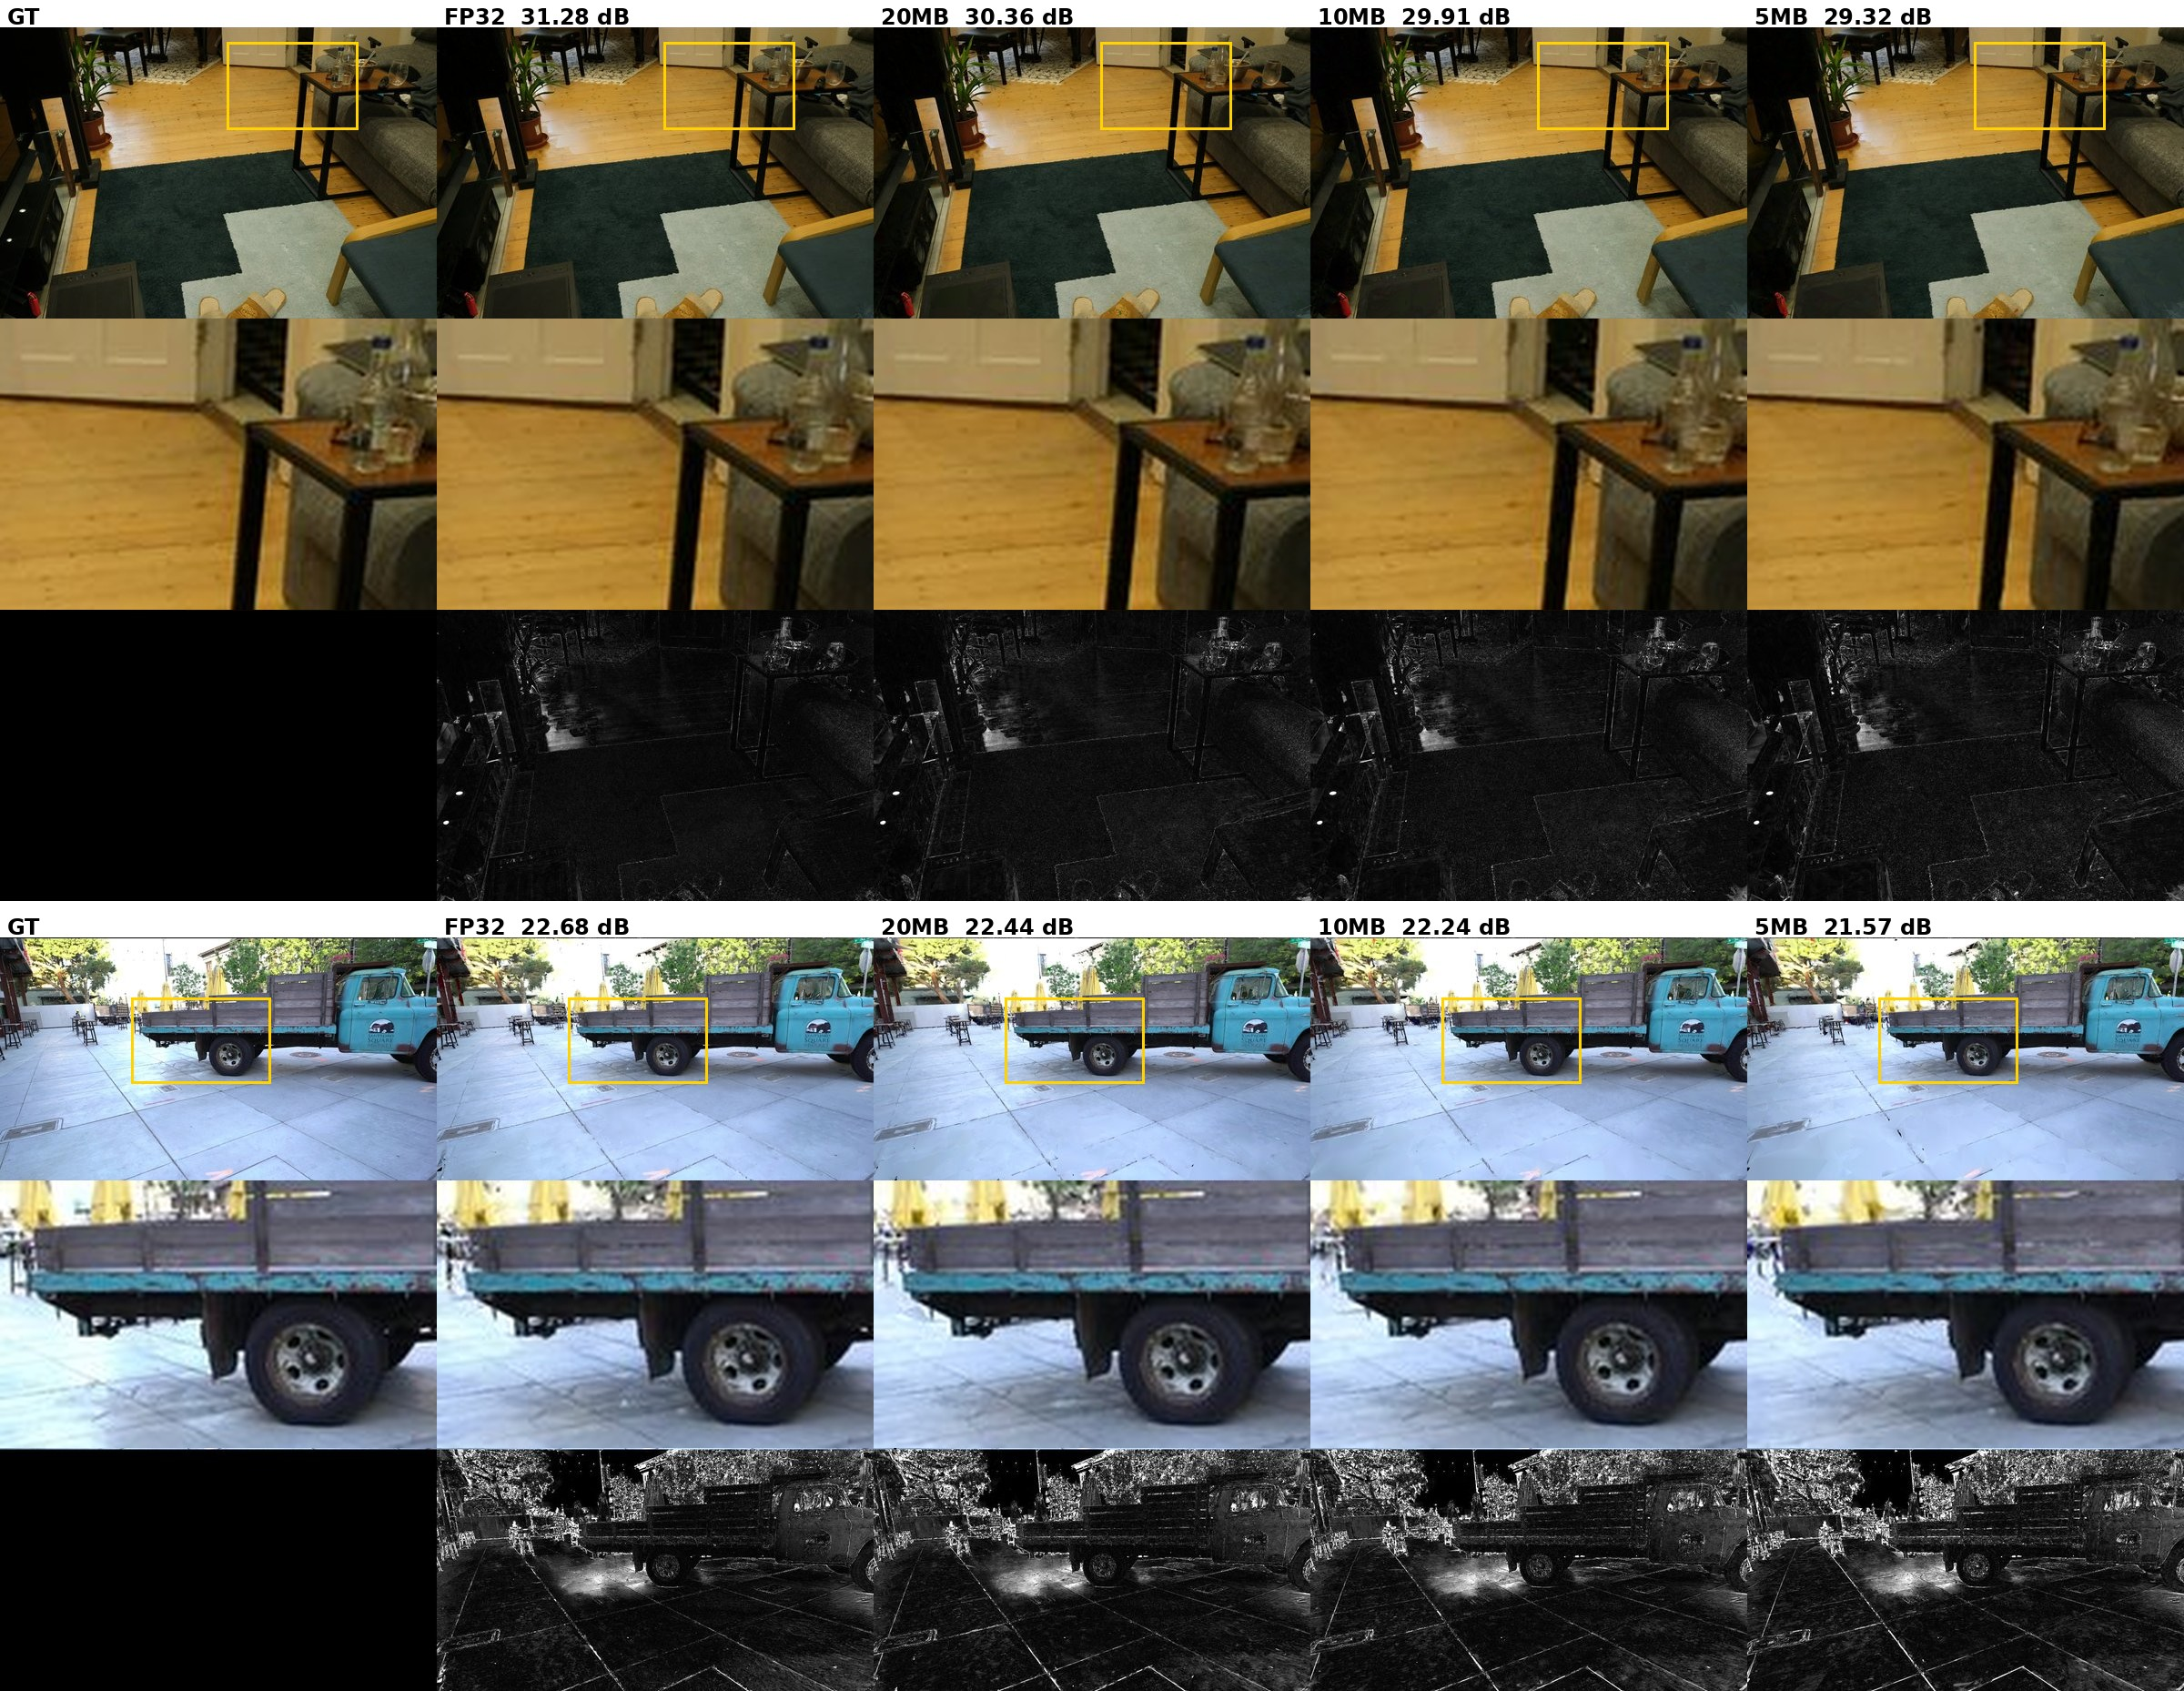
\includegraphics[width=\textwidth]{figures/fig_qualitative.jpg}\\[2pt]
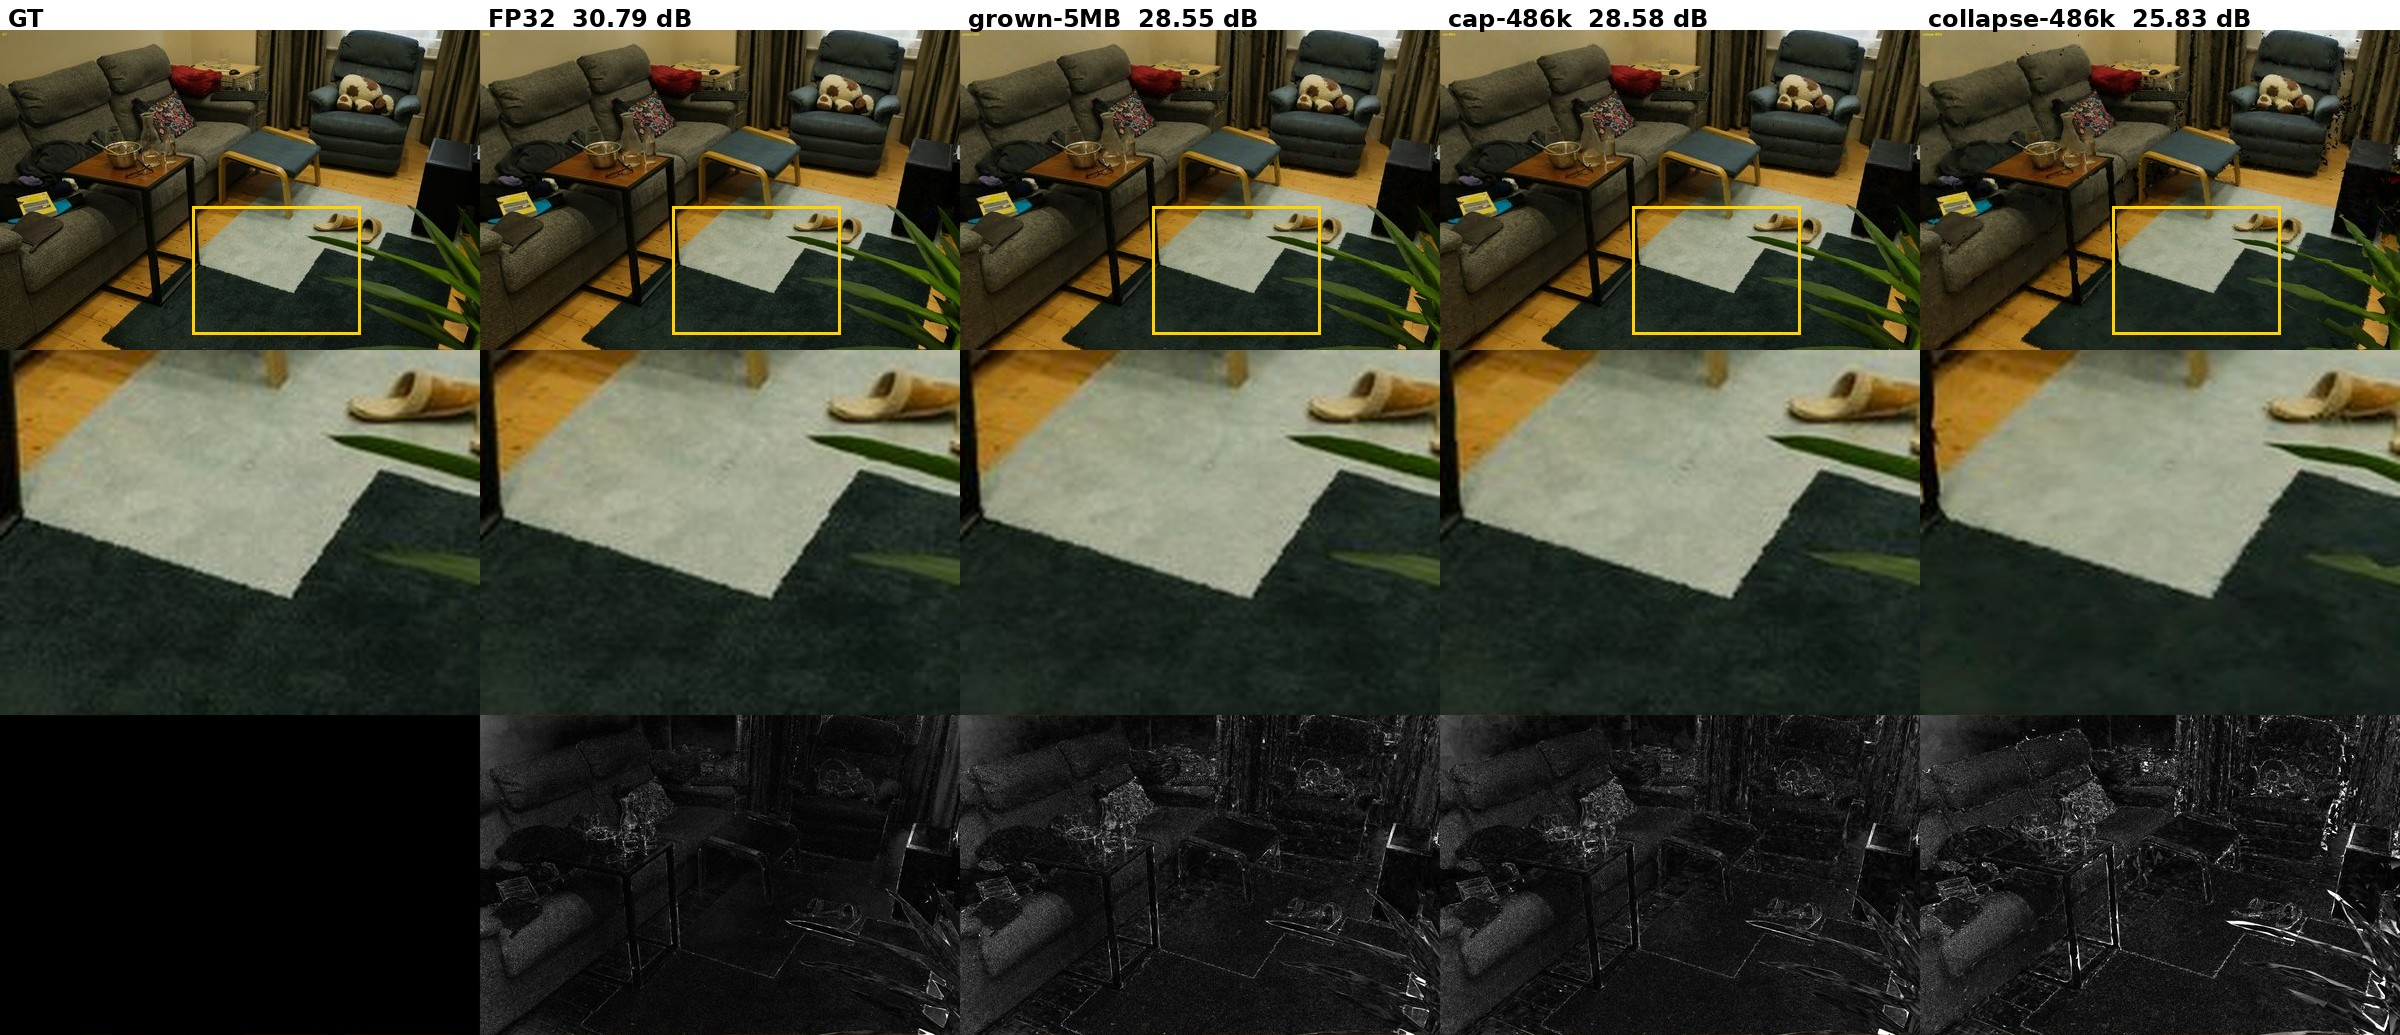
\includegraphics[width=\textwidth]{figures/fig_g0_triptych.jpg}
\caption{\textbf{Top:} decoded \BM files at three target sizes next to the ground truth and the FP32 model (room, truck): full view with PSNR, the crop enlarged, and the error map ($|$render $-$ GT$|\times4$). \textbf{Bottom:} the same vertex count reached three ways; simplification after training loses 3\dB on this view and shows holes and speckle. \TODO{camera-ready crops from the full-resolution renders; choose crops where the 5 MB file visibly fails}}
\label{fig:qual}
\end{figure*}

\noindent\textbf{Limitations.} The growth aim is one calibrated constant per capture class; it stands in for the growth of the visible-face set after stitching, which cannot be observed earlier. Indoor scenes land 5--14\% above the target and outdoor scenes at 20~MB up to 7\% below. Small objects cannot fill large targets. The trimming bound of Sec.~\ref{sec:collapse} is one-sided: it protects against undershoot from collapsing, not against the growth plan admitting too few splits. Opaque meshes are 3--4\dB below Gaussian codecs at the same file size. The entropy coders are fixed; a learned rate model is future work.
